\documentclass[10pt]{beamer}
\usepackage{kotex}
\usepackage{commath}
\usepackage{multirow}
\usepackage{multicol}
\usepackage{arydshln} % Include this package
\usepackage{bbding}

\usepackage{tikz}
\usepackage{tikz-cd}
\usetikzlibrary{math} % for calculations
\usetikzlibrary{shapes, arrows.meta, positioning, shadows}
\usetikzlibrary{arrows,shapes.geometric}  % Optional, based on your needs
\usetikzlibrary{3d, calc}
\usetikzlibrary{matrix, positioning, arrows.meta, shapes.multipart, chains}
\usetikzlibrary{decorations.pathreplacing,calligraphy}
\usetheme[progressbar=frametitle]{metropolis}
\usepackage{appendixnumberbeamer}

\usepackage{adjustbox}
\usepackage{booktabs}
\usepackage[scale=2]{ccicons}

\usepackage{tcolorbox}

\usepackage{pgfplots}
\usepgfplotslibrary{fillbetween}
\pgfplotsset{compat=1.15}
\usepgfplotslibrary{dateplot}

\usepackage{xspace}
\newcommand{\themename}{\textbf{\textsc{metropolis}}\xspace}

\usepackage[linesnumbered,ruled]{algorithm2e}
\usepackage{algpseudocode}
\usepackage{setspace}
\SetKwComment{Comment}{/* }{ */}
\SetKwProg{Fn}{Function}{:}{end}
\SetKw{End}{end}
\SetKw{DownTo}{downto}

% Define a new environment for algorithms without line numbers
\newenvironment{algorithm2}[1][]{
	% Save the current state of the algorithm counter
	\newcounter{tempCounter}
	\setcounter{tempCounter}{\value{algocf}}
	% Redefine the algorithm numbering (remove prefix)
	\renewcommand{\thealgocf}{}
	\begin{algorithm}
	}{
	\end{algorithm}
	% Restore the algorithm counter state
	\setcounter{algocf}{\value{tempCounter}}
}

\usepackage{xcolor}   % Required for specifying colors

\usepackage{listings} %Code
\renewcommand{\lstlistingname}{Code}%
\definecolor{keyword}{RGB}{255, 0, 0}
\definecolor{identifier}{RGB}{0, 0, 255}
\definecolor{comment}{RGB}{0, 128, 0}
\definecolor{string}{RGB}{163, 21, 21}

\lstdefinestyle{c}{
	language=C,
	basicstyle=\ttfamily\small,
	keywordstyle=\color{keyword},
	identifierstyle=\color{identifier},
	commentstyle=\color{comment}\itshape,
	stringstyle=\color{string},
	showstringspaces=false,
	%	numberstyle=\tiny\color{gray},
	%	numbersep=5pt,
	frame=single,
	tabsize=4,
	captionpos=b,
	breaklines=true,
	breakatwhitespace=true,
	%	numbers=left
}

\usepackage{amsthm, amsmath}


\newcommand{\cyclic}[1]{\langle #1 \rangle}
\newcommand{\uniform}{\overset{\$}{\leftarrow}}
\newcommand{\N}{\mathbb{N}}
\newcommand{\Z}{\mathbb{Z}}
\newcommand{\Q}{\mathbb{Q}}
\newcommand{\R}{\mathbb{R}}
\newcommand{\C}{\mathbb{C}}
\newcommand{\F}{\mathbb{F}}

\newcommand{\xmark}{\textcolor{red}{\XSolidBrush}}
\newcommand{\vmark}{\textcolor{green!75!black}{\CheckmarkBold}}

\newcommand{\B}{\mathbb{B}}
\newcommand{\true}{\textcolor{red}{\texttt 1}}
\newcommand{\false}{\textcolor{red}{\texttt 0}}
\newcommand{\id}{\textnormal{id}}
\title{\huge\bf Software Verification}
\subtitle{\textcolor{magenta}{\textbf{Lecture 02. OCaml Programming I}}}
% \date{\today}
\date{}
\author{\large\textcolor{cyan}{\bf Ji, Yong-Hyeon}\\ \\ \small 24. 07. 18 (Thu)}
\institute{\small
	Coding \& Optimization Together (CO2) \\
	Crypto \& Security Engineering Lab (CSE) \\
	Department of Information Security, Cryptology, and Mathematics
}
% \titlegraphic{\hfill\includegraphics[height=1.5cm]{logo.pdf}}

\begin{document}
	
	\maketitle
	
	\begin{frame}{Table of Contents}
		\setbeamertemplate{section in toc}[sections numbered]
		\tableofcontents%[hideallsubsections]
	\end{frame}
	
	\section{Motivation}
	\begin{frame}{1. Motivation}
		\url{https://www.tiobe.com/tiobe-index/}
		\begin{figure}[h!]
			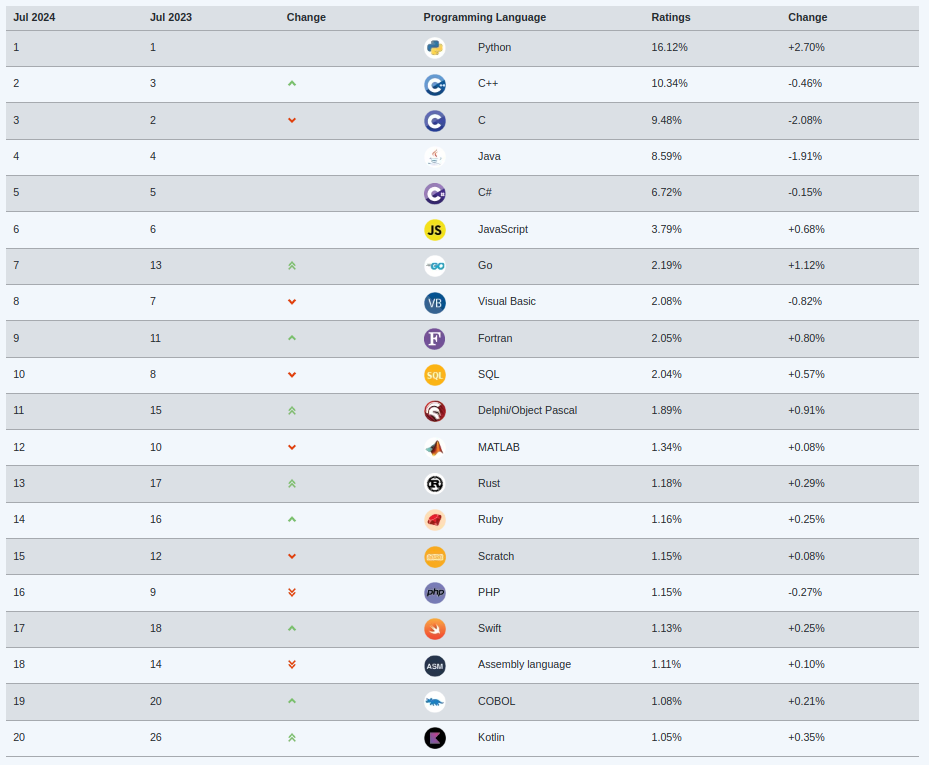
\includegraphics[scale=.35]{ranking1}
		\end{figure}
	\end{frame}
	\begin{frame}{1. Motivation}
	\begin{figure}[h!]
		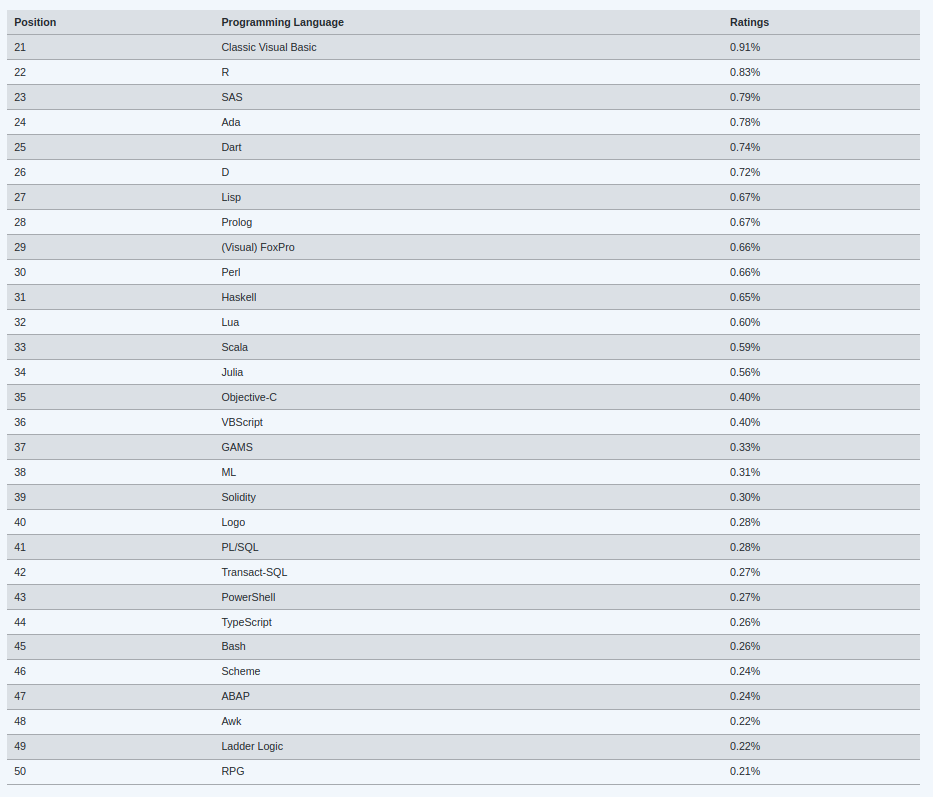
\includegraphics[scale=.35]{ranking2}
	\end{figure}
	\end{frame}
%	\begin{frame}{1. Motivation}
%		\begin{enumerate}
%			\item[3.] Current Technologies for Safe Software
%			\begin{enumerate}[(a)]
%				\item[]
%				\item Code Review
%				\item[]
%				\item Testing
%				\item[]
%				\item Debugging
%				\item[]
%				\item Simulation
%				\item[]
%				\item $\cdots$
%			\end{enumerate}
%		\end{enumerate}
%	\end{frame}

	\section{Basic OCaml Programming}
	\subsection{2.1 OCaml 기본 구성}
	\begin{frame}{2.1 OCaml 기본 구성}
		\textbf{OCaml 프로그램의 기본 단위 공식}
		
		\begin{itemize}
			\item 프로그램을 구성하는 두 가지 기본 단위
			\begin{itemize}
				\item[]
				\item[] Statement: \[
				\texttt{x = x + 1}
				\]
				\item[] Expression: \[
				\texttt{(x + y) * 2}
				\]
			\end{itemize}
		\end{itemize}
	\end{frame}

	\begin{frame}{2.1 OCaml 기본 구성}
		\textbf{$\triangleright$ OCaml 프로그램의 기본 단위 공식}
		
		\begin{itemize}
			\item 프로그램을 구성하는 두 가지 기본 단위
			\begin{itemize}
				\item[]
				\item[*] Statement \[
				\texttt{x = x + 1}
				\]
				\item[*] Expression \[
				\texttt{(x + y) * 2}
				\]
			\end{itemize}
			\item[]
			\item[]
			\item[]
			\begin{itemize}
				\item[]
				\item[]
				\begin{itemize}
					\item[] 
					\item[]
				\end{itemize}
				\item[]
				\item[]
				\begin{itemize}
					\item[]
					\item[]
				\end{itemize}
			\end{itemize}
		\end{itemize}
	\end{frame}
	
	\begin{frame}{2.1 OCaml 기본 구성}
		
		\textbf{$\triangleright$ OCaml 프로그램의 기본 단위 공식}
	\begin{itemize}
		\item 프로그램을 구성하는 두 가지 기본 단위
		\begin{itemize}
			\item[]
			\item[*] Statement (명령문): 기계 상태를 변경 \[
			\texttt{x = x + 1}
			\]
			\item[*] Expression (식): 상태 변경 없이 값을 계산 \[
			\texttt{(x + y) * 2}
			\]
		\end{itemize}
		\item[]
		\item[]
		\item[]
		\begin{itemize}
			\item[]
			\item[]
			\begin{itemize}
				\item[] 
				\item[]
			\end{itemize}
			\item[]
			\item[]
			\begin{itemize}
				\item[]
				\item[]
			\end{itemize}
		\end{itemize}
	\end{itemize}
\end{frame}

	\begin{frame}{2.1 OCaml 기본 구성}
		\textbf{$\triangleright$ OCaml 프로그램의 기본 단위 공식}
		
		\begin{itemize}
			\item 프로그램을 구성하는 두 가지 기본 단위
			\begin{itemize}
				\item[]
				\item[*] Statement (명령문): 기계 상태를 변경 \[
				\texttt{x = x + 1}
				\]
				\item[*] Expression (식): 상태 변경 없이 값을 계산 \[
				\texttt{(x + y) * 2}
				\]
			\end{itemize}
			\item 프로그래밍 언어를 구분하는 한가지 기준:
			\begin{itemize}
				\item[]
				\item[*] 명령문을 중심으로 프로그램을 작성
				\begin{itemize}
					\item[-] C, C++, Java, Python, JavaScript, etc.
					\item[-] ``Imperative Languages''
				\end{itemize}
				\item[]
				\item[*] 식을 중심으로 프로그램을 작성
				\begin{itemize}
					\item[-] ML, Haskell, Scala, Lisp, etc.
					\item[-] ``Functional Programming''
				\end{itemize}
			\end{itemize}
		\end{itemize}
	\end{frame}

	\begin{frame}{2.1 OCaml 기본 구성}
		\textbf{$\triangleright$ OCaml 프로그램의 기본 구조}
		
		\begin{itemize}
			\item 값 정의들의 나열 \begin{align*}
				\texttt{let}\ x_1 &= e_1\\
				\texttt{let}\ x_2 &= e_2\\
				&\vdots \\
				\texttt{let}\ x_n &= e_n\\
			\end{align*}
			\item[*] 식 $e_1,e_2,\dots,e_n$을 순차적으로 계산
			\item[]
			\item[*] 변수 $x_i$는 식 $e_i$의 값을 지칭 (assignment vs binding)
			\item[]
			\item[]
		\end{itemize}
	\end{frame}

\begin{lstlisting}[style=ocaml]
let hello = "Hello"
let world = "World"
let helloworld = hello ^ " " ^ world
let _ = print_endline helloworld
\end{lstlisting}

Compile
\begin{lstlisting}[style=zsh]
@:~$>ocaml helloworld.ml
\end{lstlisting}

OCaml REPL(Real-Eval-Print Loop)
\begin{lstlisting}[style=zsh]
@:~$>ocaml

# #use "helloworld.ml";;
val hello : string = "Hello"
val world : string = "World"
val helloworld : string = "Hello World"
Hello World
- : unit = ()
# exit 1;;
\end{lstlisting}
	\newpage
	\begin{frame}{2.1 OCaml 기본 구성}
		\textbf{$\triangleright$ Arithmetic Expression (산술식)}
		
		\begin{itemize}
			\item 정수와 실수
		\end{itemize}
		\begin{tcolorbox}[colback=backcolor]\ttfamily
			\# 1 + 2 * 3;;\\
			- : int = 7\\
			\# 1.1 +. 2.2 *. 3.3;;\\
			- : float = 8.36
		\end{tcolorbox}
		\begin{itemize}
			\item[] 정수값을 위한 산술 연산자 \[
			+,\quad -,\quad*,\quad/,\quad\texttt{mod}
			\]
			\item[] 실수값을 위한 산술 연산자 \[
			+.,\quad -.,\quad*.,\quad/.,\quad\texttt{mod\_float(.,.)}
			\]
			\item[]
		\end{itemize}
	\end{frame}

	\begin{frame}{2.1 OCaml 기본 구성}
		\textbf{$\triangleright$ Arithmetic Expressions (산술식)}
		
		\begin{itemize}
			\item 정수 타입과 실수 타입을 명확히 구분하자
		\end{itemize}
		 \begin{tcolorbox}[colback=backcolor]\ttfamily
			\# 3 + 2.0;; \\
			Error: This expression has type float but an expression was expected of type
			int\\
			\# 3 + int\_of\_float 2.0;;\\
			- : int = 5
		\end{tcolorbox}	
		\begin{itemize}
			\item[] 
			\item[] 
			\item[] 
			\item[] 
			\item[] 
		\end{itemize}
	\end{frame}

	\begin{frame}{2.1 OCaml 기본 구성}
		\textbf{$\triangleright$ Boolean Expressions (논리식)}
		
		\begin{itemize}
			\item 논리값
		\end{itemize}
		\begin{tcolorbox}[colback=backcolor]\ttfamily
			\# true;; \\
			- : bool = true\\
			\# false;; \\
			- : bool = false
		\end{tcolorbox}
		\begin{itemize}
			\item 비교 연산자 (산술식 $\to$ 논리식)
		\end{itemize}
		\begin{tcolorbox}[colback=backcolor]\ttfamily
			\# 1 = 2;; \\
			- : bool = false\\
			\# 1 <> 2;; \\
			- : bool = true\\
			\# 2 <= 2;; \\
			- : bool = true
		\end{tcolorbox}
	\end{frame}

	\begin{frame}{2.1 OCaml 기본 구성}
		\textbf{$\triangleright$ Boolean Expressions (논리식)}
		
		\begin{itemize}
			\item 논리 연산자 (논리식 $\to$ 논리식)
		\end{itemize}
		\begin{tcolorbox}[colback=backcolor]\ttfamily
			\# true \&\& (false || not false);; \\
			- : bool = true\\
			\# (2 > 1) \&\& (3 > 2);; \\
			- : bool = false
		\end{tcolorbox}
		\begin{itemize}
			\item[] 
			\item[] 
			\item[] 
			\item[] 
			\item[] 
			\item[] 
			\item[] 
		\end{itemize}
	\end{frame}

	\begin{frame}{2.1 OCaml 기본 구성}
		\textbf{$\triangleright$ Primitive Values (기본값)}
		
		\begin{itemize}
			\item OCmal은 \begin{itemize}
				\item[-] integer (정수) 
				\item[-] float (실수)
				\item[-] boolean (논리)
				\item[-] character (문자)
				\item[-] string (문자열)
				\item[-] unit (유닛)
			\end{itemize}을 제공
		\end{itemize}
		\begin{tcolorbox}[colback=backcolor]\ttfamily
			\# 'c';; \\
			- : char = 'c'\\
			\# "Objecive " \^{} "Caml";; \\
			- : string = "Objective Caml"\\
			\# ();;\\
			- : unit = ()
		\end{tcolorbox}
	\end{frame}

	\begin{frame}{2.1 OCaml 기본 구성}
		\textbf{$\triangleright$ Conditional Expression (조건식)}	
		\[
		\texttt{if $e_1$ then $e_2$ else $e_3$}
		\]
		\begin{tcolorbox}[colback=backcolor]\ttfamily
		\# if 1 then 2 else 3;;
		\end{tcolorbox}
		\begin{itemize}
			\item[] 
			\item[] 
			\item[] 
			\item[] 
			\item[] 
			\item[] 
			\item[] 
			\item[] 
		\end{itemize}
	\end{frame}
	\begin{frame}{2.1 OCaml 기본 구성}
		\textbf{$\triangleright$ Conditional Expression (조건식)}	
		\[
		\texttt{if $e_1$ then $e_2$ else $e_3$}
		\]
		\begin{itemize}
			\item $e_1$은 반드시 논리식이어야 함. 즉 $e_1$의 값은 true or false
		\end{itemize}
		\begin{tcolorbox}[colback=backcolor]\ttfamily
			\# if 1 then 2 else 3;;\\
			Error: This expression has type int but an expression was expected of type
			bool
			because it is in the condition of an if-statement
		\end{tcolorbox}
		\begin{itemize}
			\item[] 
			\item[] 
			\item[] 
		\end{itemize}
	\end{frame}
	
	\begin{frame}{2.1 OCaml 기본 구성}
		\textbf{$\triangleright$ Conditional Expression (조건식)}
		\begin{itemize}
			\item 조건식의 값은 $e_1$ 값에 따라서 결정
		\end{itemize}
		\begin{tcolorbox}[colback=backcolor]\ttfamily
			\# if 2 $>$ 1 then 0 else 1;;\\
			- : int = 0 \\
			\# if 2 < 1 then 0 else 1;; \\
			- : int = 1
		\end{tcolorbox}
		\begin{itemize}
			\item $e_2$와 $e_3$는 타입이 같아야 함
		\end{itemize}
		\begin{tcolorbox}[colback=backcolor]\ttfamily
			\# if true then 1 else true;;\\
			Error: This expression has type bool but an expression was expected of type
			int
		\end{tcolorbox}
		\begin{itemize}
			\item[]
		\end{itemize}
	\end{frame}

	\begin{frame}{2.1 OCaml 기본 구성}
		\textbf{$\triangleright$ \textcolor{red}{Function Expression} (함수식)}
		\[
		\texttt{fun $x$ -> $e$}
		\] 
		\begin{itemize}
			\item 함수의 예:
			\begin{itemize}
				\item[*] \texttt{fun $x$ -> $x+1$}
				\item[*] \texttt{fun $y$ -> $y*y$}
				\item[*] \texttt{fun $x$ -> if $x>0$ then $x+1$ else $x*x$}
				\item[*] \texttt{fun $x$ -> fun $y$ -> $x+y$}
				\item[*] \texttt{fun $x$ -> fun $y$ -> fun $z$ -> $x+y+z$}
			\end{itemize}
			\item[]
			\item Syntactic Sugar \[
			\texttt{fun $x_1\ \dots\ x_n$\ ->\ $e$}
			\]
			\begin{itemize}
				\item[*] \texttt{fun $x$ $y$ -> $x+y$}
				\item[*] \texttt{fun $x$ $y$ $z$ -> $x+y+z$}
			\end{itemize}
		\end{itemize}
	\end{frame}
\begin{itemize}
	\item[]
	\item[]
	\item[]
\end{itemize}
\begin{lstlisting}[style=zsh]
@:~$>ocaml

# let f = fun x y -> x + y;;
val f : int -> int -> int = <fun>
# f 1 2;
- : int = 3
# let g = f 1;
# g 2;;
- : int = 3
\end{lstlisting}

\newpage
\ \\ \textbf{\Huge Currying} \begin{table}[h!]\centering\begin{tabular}{|cc|c|} \hline
		$P$ & $Q$ & $P\land Q$ \\ \hline
		$\false$ & $\false$ & $\false$ \\ \hline
		$\false$ & $\true$ & $\false$ \\ \hline
		$\true$ & $\false$ & $\false$ \\ \hline
		$\true$ & $\true$ & $\true$ \\ \hline
	\end{tabular}
\end{table}
\begin{center}\begin{minipage}{.48\textwidth}\centering\adjustbox{scale=.8}{
			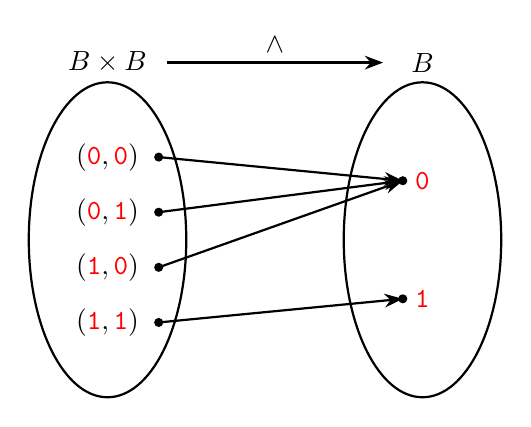
\begin{tikzpicture}
				% Draw the sets A and B
				\draw[thick] (-2,0) ellipse (1 and 2);
				\draw[thick] ( 2,0) ellipse (1 and 2);
				
				% Labels for sets
				\node at (-2, 2.25) {$\B\times\B$};
				\node at ( 2, 2.25) {$\B$};
				
				% Draw the arrows representing the function
				\draw[-Stealth, thick] (-1.25, 2.25) -- (1.5,2.25) node[midway, above] {$\land$};
				
				\node at (-2,  1.05) {$(\false,\false)$};
				\node at (-2,   .35) {$(\false,\true)$};
				\node at (-2, - .35) {$(\true,\false)$};
				\node at (-2, -1.05) {$(\true,\true)$};
				\draw[fill] (-1.35, 1.05) circle (.05);
				\draw[fill] (-1.35,  .35) circle (.05);
				\draw[fill] (-1.35, -.35) circle (.05);
				\draw[fill] (-1.35,-1.05) circle (.05);
				
				\node at (2,  .75) {$\false$};
				\node at (2, -.75) {$\true$};
				\draw[fill] (1.75, .75) circle (.05);
				\draw[fill] (1.75,-.75) circle (.05);
				
				\draw[-Stealth, thick] (-1.35, 1.05) -- (1.75, .75);
				\draw[-Stealth, thick] (-1.35, .35) -- (1.75, .75);
				\draw[-Stealth, thick] (-1.35, -.35) -- (1.75, .75);
				\draw[-Stealth, thick] (-1.35, -1.05) -- (1.75, -.75);
		\end{tikzpicture}}\\
	\end{minipage}\begin{minipage}{.48\textwidth}\centering\adjustbox{scale=.8}{
			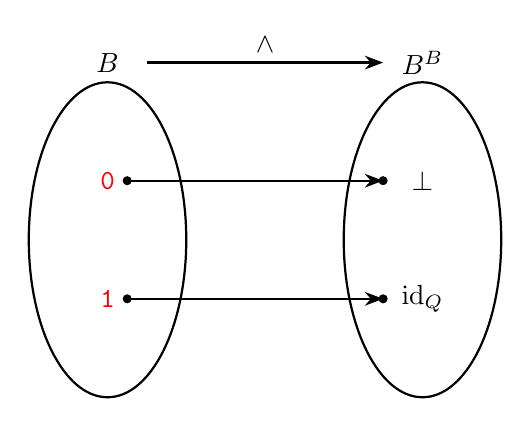
\begin{tikzpicture}
				% Draw the sets A and B
				\draw[thick] (-2,0) ellipse (1 and 2);
				\draw[thick] ( 2,0) ellipse (1 and 2);
				
				% Labels for sets
				\node at (-2, 2.25) {$\B$};
				\node at ( 2, 2.25) {$\B^{\B}$};
				
				% Draw the arrows representing the function
				\draw[-Stealth, thick] (-1.5, 2.25) -- (1.5,2.25) node[midway, above] {$\land$};
				
				\node at (-2, .75) {$\false$};
				\node at (-2, -.75) {$\true$};
				\draw[fill] (-1.75,.75) circle (.05);
				\draw[fill] (-1.75,-.75) circle (.05);
				
				\node at (2, .75) {$\bot$};
				\node at (2, -.75) {$\id_Q$};
				\draw[fill] (1.5,.75) circle (.05);
				\draw[fill] (1.5,-.75) circle (.05);
				
				\draw[-Stealth, thick] (-1.75, .75) -- (1.5, .75);
				\draw[-Stealth, thick] (-1.75, -.75) -- (1.5, -.75);
		\end{tikzpicture}}\\
\end{minipage}\end{center}
\newpage
%	\subsection{2.2 리스트와 재귀함수}
%	\begin{frame}{2.2 리스트와 재귀함수}
%		content...
%	\end{frame}
%
%	
%	\subsection{2.3 고차 함수}
%	\begin{frame}{2.3 고차 함수}
%		content...
%	\end{frame}
%	
%	
%	\subsection{2.4 사용자 정의 타입}
%	\begin{frame}{2.4 사용자 정의 타입}
%		content...
%	\end{frame}

	\section{Advanced OCaml Programming}
	
	\newpage
	{\setbeamercolor{palette primary}{fg=black, bg=-blue}
		\begin{frame}[standout]
			To be continue ...
		\end{frame}
	}
	
	%\appendix
	%
	%\begin{frame}[fragile]{Backup slides}
	%  Sometimes, it is useful to add slides at the end of your presentation to
	%  refer to during audience questions.
	%
	%  The best way to do this is to include the \verb|appendixnumberbeamer|
	%  package in your preamble and call \verb|\appendix| before your backup slides.
	%
	%  \themename will automatically turn off slide numbering and progress bars for
	%  slides in the appendix.
	%\end{frame}
	%
	%\begin{frame}[allowframebreaks]{References}
	%
	%  \bibliography{demo}
	%  \bibliographystyl{abbrv}
	%
	%\end{frame}
	
\end{document}
